\subsection{Adapter (\textit{o Wrapper})}
\label{adapter}

\textbf{Scopo}: Strutturale \\
\textbf{Raggio d'azione}: Classi e oggetti

\paragraph{Definizione}
Il patter Adapter permette di convertire l'interfaccia di una classe in un'altra interfaccia richiesta dal client.

Consente a classi diverse di cooperare insieme quando ciò non sarebbe possibile a causa di interfacce incompatibili

\paragraph{Problema} A volte una classe preesistente, progettata per essere riutilizzata, non può essere riusata perché incompatibile con l'interfaccia richiesta dall'applicazione.

\begin{figure}[H]
    \centering
    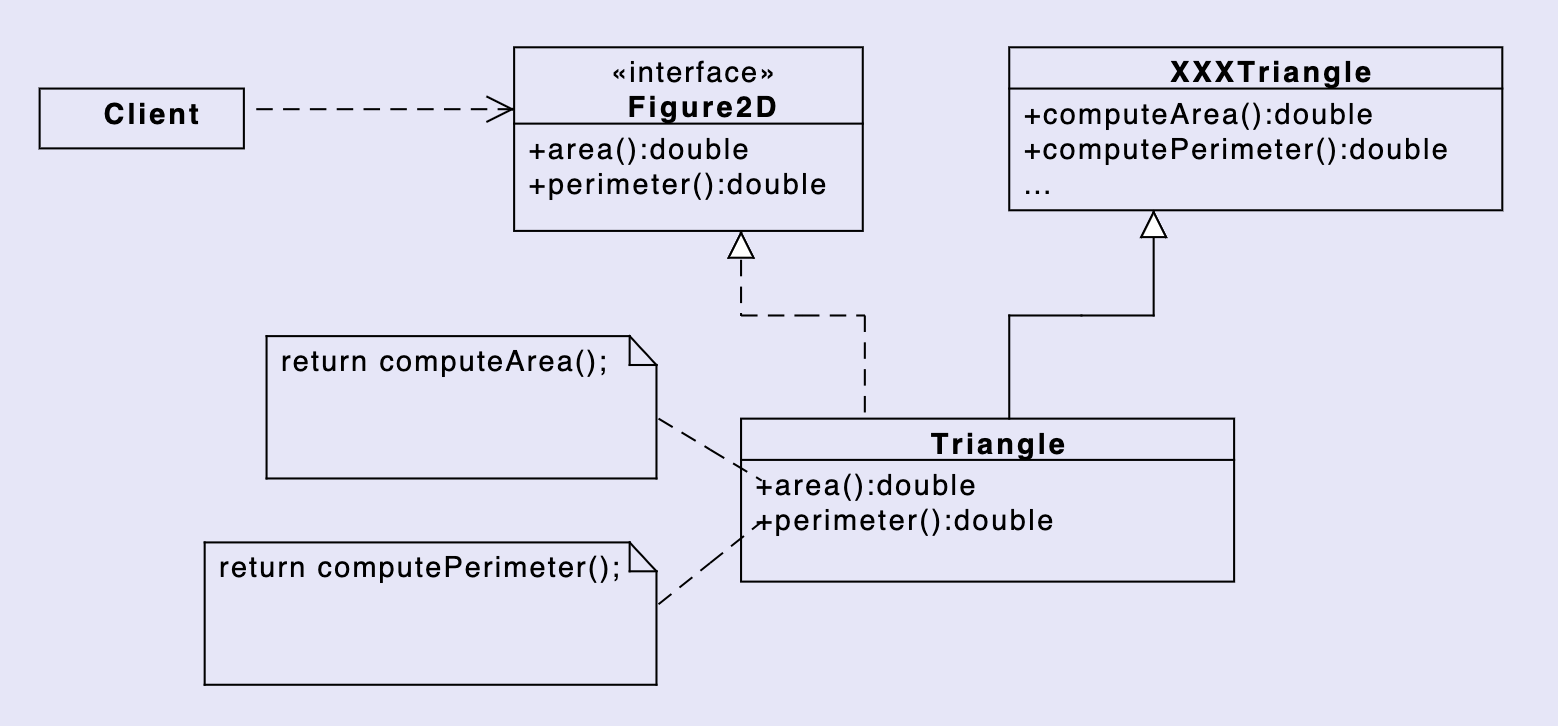
\includegraphics[width=1\linewidth]{assets/pattern/adapter/class-adapter.png}
    \caption{Esempio di Class Adapter}
\end{figure}

Nell’esempio, la classe XXXTriangle non può essere riusata dove ci si aspetta l’interfaccia Figure2D perché non è compatibile con essa.

\paragraph{Soluzione} Pensare di modificare XXXTriangle per renderla conforme a Figure2D non è una buona soluzione (si legherebbe al contesto specifico e il codice sorgente potrebbe non essere disponibile).

Si introduce una classe Triangle che sia al contempo erede di entrabe XXXTriangle e Figure2D. L'implementazione dei metodi di Figure2D sfrutta quelli di XXXTriangle.

\begin{figure}[H]
    \centering
    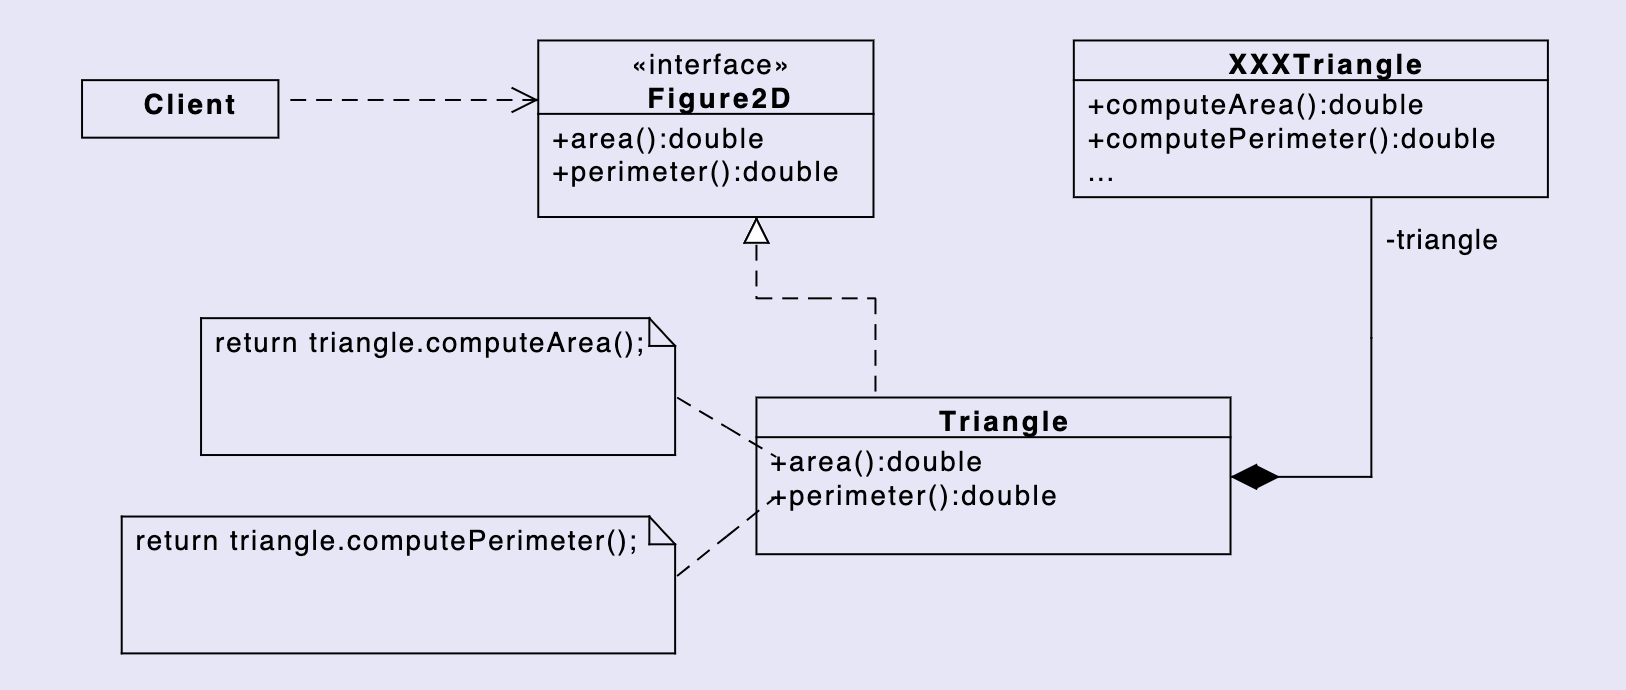
\includegraphics[width=1\linewidth]{assets/pattern/adapter/object-adapter.png}
    \caption{Esempio di Object Adapter}
\end{figure}

È possibile introdurre la classe Triangle anche di modo che faccia riferimento ad un oggetto (istanza di XXXTriangle) e vada ad implementare l'interfaccia Figure2D delegando l'esecuzione all'oggetto incapsulato.

\paragraph{Struttura e Conseguenze} Il pattern è composto dai seguenti partecipanti:
\begin{itemize}
    \item \textbf{Target} (Figure2D): definisce l'interfaccia specifica del dominio utilizzata dal client
    \item \textbf{Client}: collabora con oggetti compatibili con l'intefaccia Target
    \item \textbf{Adaptee} (XXXTriangle): individua un'interfaccia che deve essere adattata.
    \item \textbf{Adapter} (Triangle): adatta l'interfaccia Adaptee al'interfaccia Target
\end{itemize}

È bene precisare che i client invocano le operazioni su in'istanza di Adapter, il quale invoca operazioni di Adaptee per soddisfare la richiesta

\textbf{Class Adapter}
\begin{itemize}
    \item Adatta l'interfaccia Adaptee all'interfaccia Target basandosi su una classe concreta.
    \item Non può essere utilizzata se Adaptee è astratta oppure è un'interfaccia.
    \item Consente ad Adapter di sovrascrivere parte del comportamento di Adaptee essendo una sua sottoclasse
    \item Non occorrono ulteriori indirezioni per raggiungere l'oggetto adattato
\end{itemize}

\textbf{Object Adapter}
\begin{itemize}
    \item Permette ad un singolo Adapter di operare con Adaptee e le sue sottoclassi, se esistono. Può in tal caso aggiungere funzionalità a tutti gli Adaptee
    \item Rende difficile sovrascrivere il comportamento di Adaptee non essendo una sua sottoclasse
    \item Aggiunge un livello di indirezione per raggiungere l'oggetto adattato.
\end{itemize}

\begin{figure}[H]
    \centering
    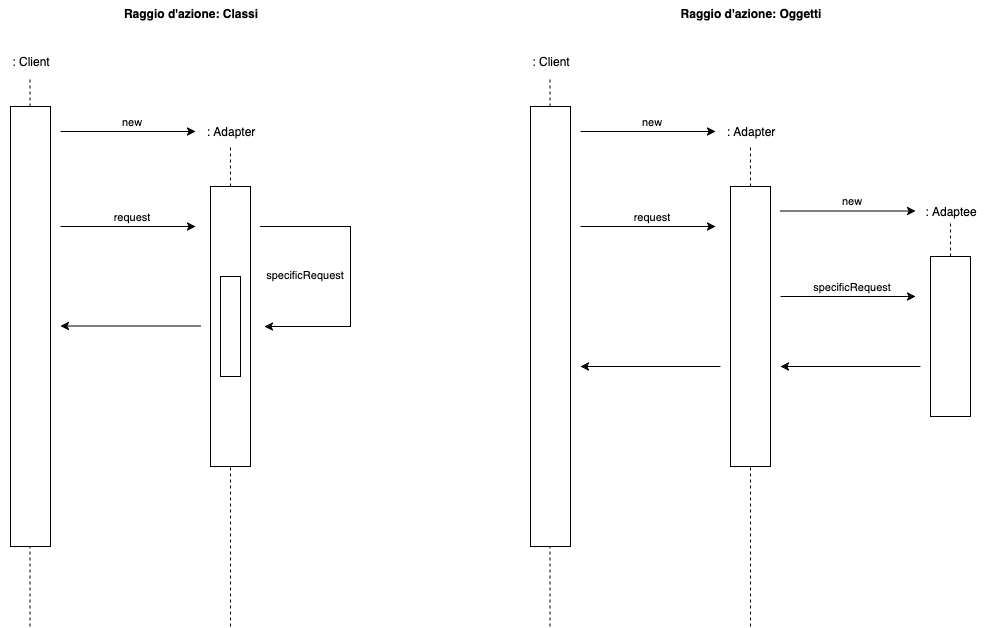
\includegraphics[width=1\linewidth]{assets/pattern/adapter/adapter-activity.drawio.png}
    \caption{Activity diagram raggio d'azione}
\end{figure}

\newpage